\documentclass[12pt]{article}
\usepackage[utf8]{inputenc}

\usepackage{lmodern}

\usepackage{enumitem}
\usepackage[margin=2cm]{geometry}

\usepackage{amsmath, amsfonts, amssymb}
\usepackage{graphicx}
%\usepackage{subfigure}
\usepackage{tikz}
\usepackage{pgfplots}
\usepackage{multicol}

\usepackage{comment}
\usepackage{url}
\usepackage{calc}
\usepackage{subcaption}
\usepackage[indent=0pt]{parskip}
\usepackage{animate}

\usepackage{array}
\usepackage{blkarray,booktabs, bigstrut}
\usepackage{bigints}

\pgfplotsset{compat=1.16}

% MATH commands
\newcommand{\ga}{\left\langle}
\newcommand{\da}{\right\rangle}
\newcommand{\oa}{\left\lbrace}
\newcommand{\fa}{\right\rbrace}
\newcommand{\oc}{\left[}
\newcommand{\fc}{\right]}
\newcommand{\op}{\left(}
\newcommand{\fp}{\right)}

\newcommand{\bi}{\mathbf{i}}
\newcommand{\bj}{\mathbf{j}}
\newcommand{\bk}{\mathbf{k}}
\newcommand{\bF}{\mathbf{F}}

\newcommand{\mR}{\mathbb{R}}

\newcommand{\ra}{\rightarrow}
\newcommand{\Ra}{\Rightarrow}

\newcommand{\sech}{\mathrm{sech}\,}
\newcommand{\csch}{\mathrm{csch}\,}
\newcommand{\curl}{\mathrm{curl}\,}
\newcommand{\dive}{\mathrm{div}\,}

\newcommand{\ve}{\varepsilon}
\newcommand{\spc}{\vspace*{0.5cm}}

\DeclareMathOperator{\Ran}{Ran}
\DeclareMathOperator{\Dom}{Dom}

\newcommand{\exo}[1]{\noindent\textcolor{red}{\fbox{\textbf{Problem {#1}}}\hrulefill}\\}
\newcommand{\qu}[4]{\noindent\textcolor{#4}{\fbox{\textbf{Section {#1} | Problem {#2}}} \hrulefill{{\fbox{\textbf{{#3} Points}}}}\\}}

\newcommand{\semester}{Spring 2023}

\newcommand{\CVup}{%

\begin{tikzpicture}
\draw[black, <->, >=latex] (-0.33, 0.5) .. controls (-0.125, 0) and (0.125, 0) .. (0.33, 0.5);
\end{tikzpicture}}

\newcommand{\CVupInc}{%
\begin{tikzpicture}
\draw[black, ->, >=latex] (0,0) .. controls (0.2, 0) and (0.4, 0.2) .. (0.5, 0.5);
\end{tikzpicture}}

\newcommand{\CVupDec}{%
\begin{tikzpicture}[rotate=270]
\draw[black, ->, >=latex] (0,0) .. controls (0.2, 0) and (0.4, 0.2) .. (0.5, 0.5);
\end{tikzpicture}}

\newcommand{\CVdown}{%
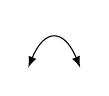
\begin{tikzpicture}
\draw[black, <->, >=latex] (-0.33, -0.5) .. controls (-0.125, 0) and (0.125, 0) .. (0.33, -0.5);
\end{tikzpicture}}

\newcommand{\CVdownInc}{%
\begin{tikzpicture}
\draw[black, ->, >=latex] (-0.5, -0.5) .. controls (-0.5, -0.3) and (-0.5, -0.1) .. (0,0);
\end{tikzpicture}}

\newcommand{\CVdownDec}{%
\begin{tikzpicture}[rotate=-90]
\draw[black, ->, >=latex] (-0.5, -0.5) .. controls (-0.5, -0.3) and (-0.5, -0.1) .. (0,0);
\end{tikzpicture}}

\begin{document}
	\noindent \hrulefill \\
	MATH-241 \hfill Pierre-Olivier Paris{\'e}\\
	Solutions Section 1-6 \hfill \semester \\\vspace*{-1cm}
	
	\noindent\hrulefill
	
	\spc
	
	\exo{8}
	\\
	Let's call $L$ the limit.
	We have
		\begin{align*}
		L &= \Big( \lim_{t \ra 2} \frac{t^2 - 2}{t^3 - 3t + 5} \Big)^2 \tag{Power Rule} \\
		&= \Big( \frac{\lim_{t \ra 2} t^2 - 2}{\lim_{t \ra 2} t^3 - 3t + 5} \Big)^2 \tag{Quotient Rule} \\
		&= \Big( \frac{\lim_{t \ra 2} t^2 - \lim_{t \ra 2} 2}{\lim_{t \ra 2} t^3 -  \lim_{t \ra 2} 3t + \lim_{t \ra 2} 5} \Big)^2 \tag{Sum \& Difference Rules}  \\
		&= \Big( \frac{(\lim_{t \ra 2} t)^2 - \lim_{t \ra 2} 2}{(\lim_{t \ra 2} t)^3 -  3\lim_{t \ra 2} t + \lim_{t \ra 2} 5} \Big)^2 \tag{Product \& Power rules} \\
		&= \Big( \frac{2^2 - 2}{2^3 - 6 + 5} \Big)^2 = \frac{4}{49} .
		\end{align*}
	So the limit is $L = 4/49$.
	
	\spc
	
	\exo{12}
	\\
	Unfortunately, we can't use the quotient rule because we have an indetermination $0/0$. Therefore, we have to check if we can rewrite the expression in the limit into another way so we can use the limit rules.
	
	For $x \neq -3$, we have
		\begin{align*}
		\frac{x^2 + 3x}{x^2 - x - 12} = \frac{x (x + 3)}{(x - 4) (x + 3)} = \frac{x}{x - 4} .
		\end{align*}
	Since $\lim_{x \ra -3} x - 4 = -7 \neq 0$, we can use the quotient rule and get
		\begin{align*}
		\lim_{x \ra -3} \frac{x^2 + 3x}{x^2 - x - 12} = \lim_{x \ra -3} \frac{x}{x - 4} = \frac{\lim_{x \ra -3} x}{\lim_{x \ra -3} x - 4} = \frac{3}{7} .
		\end{align*}
		
	\spc
	
	\exo{22}
	\\
	If we would use the quotient rule, we would get $0/0$. Since this is undefined, we most remove this undetermination.
	
	For $x \neq 2$, we have
		\begin{align*}
		\frac{\sqrt{4u + 1} - 3}{u - 2} = \op \frac{\sqrt{4u + 1} - 3}{u - 2} \fp \op \frac{\sqrt{4u + 1} + 3}{\sqrt{4u + 1} + 3} \fp = \frac{4u + 1 - 9}{(u - 2) (\sqrt{4u + 1} + 3} = 4 \frac{u - 2}{(u - 2) (\sqrt{4u + 1} + 3)}
		\end{align*}
	and simplifying $u - 2$, we obtain
		\begin{align*}
		\frac{\sqrt{4u + 1} - 3}{u - 2} = \frac{4}{\sqrt{4u + 1} + 3}
		\end{align*}
	Now, using the power rule and the sum rule, we see that
		\begin{align*}
		\lim_{u \ra 2} \sqrt{4u + 1} + 3 = \sqrt{\lim_{u \ra 2} 4u + 1} + 3 = \sqrt{8 + 1} + 3 = 6 .
		\end{align*}
	Since $6$ is different from zero, we can use the quotient rule! We therefore obtain
		\begin{align*}
		\lim_{u \ra 2} \frac{\sqrt{4u + 1} - 3}{u - 2} = \lim_{u \ra 2} \frac{4}{\sqrt{4u + 1} + 3} = \frac{\lim_{u \ra 2} 4}{\lim_{u \ra 4} \sqrt{4u + 1} + 3} = \frac{4}{6} = \frac{2}{3} .
		\end{align*}
		
	\spc
	
	\exo{26}
	\\
	We have
		\begin{align*}
		\frac{1}{t} - \frac{1}{t^2 + t} = \frac{1}{t} - \frac{1}{(t + 1)t} = \frac{t + 1 - 1}{t (t + 1)} = \frac{1}{t + 1} .
		\end{align*}
	So the limit is
		\begin{align*}
		\lim_{t \ra 0} \Big( \frac{1}{t} - \frac{1}{t^2 + t} \Big) = \lim_{t \ra 0} \frac{1}{1 + t} = 1 .
		\end{align*}
	
	\spc
	
	\exo{36}
	\\
	Since $-1 \leq \sin A \leq 1$ for any real number $A$, we know that $-1 \leq \sin \op \frac{\pi}{x} \fp \leq 1$. Therefore, multiplying by $\sqrt{x^3 + x^2}$, we obtain
		\begin{align*}
		- \sqrt{x^3 + x^2} \leq \sqrt{x^3 + x^2} \sin \op \frac{\pi}{x} \fp \leq \sqrt{x^3 + x^2} .
		\end{align*}
	
	Using the power rule and the sum rule, we have
		\begin{align*}
		\lim_{x \ra 0} \sqrt{x^3 + x^2} = 0 = \lim_{x \ra 0} - \sqrt{x^3 + x^2} .
		\end{align*}
	Therefore, by the Squeeze Theorem, we can conclude that
		\begin{align*}
		\lim_{x \ra 0} \sqrt{x^3 + x^2} \sin \op \frac{\pi}{x} \fp = 0 .
		\end{align*}
		
	\spc
	
	\exo{42}
	\\
	We have to check if the limit from the left is the same as the limit from the right. 
	
	For the limit from the left, we will approach $-6$ with numbers $x$ less than $-6$. Therefore, $x + 6 < 0$ for $x < -6$ and $|x + 6| = - (x + 6) = -x - 6$. Therefore, we get
		\begin{align*}
		\lim_{x \ra -6^-} \frac{2x + 12}{|x + 6|} = \lim_{x \ra -6^-} 2 \frac{x + 6}{-(x + 6)} = \lim_{x \ra -6^-} -2 = -2 .
		\end{align*}
		
	For the limit from the right, we will approach $-6$ with numbers $x$ greater than $-6$. This means $x + 6 > 0$ (when $x > -6$) and therefore $|x + 6| = x+ 6$. We then get
		\begin{align*}
		\lim_{x \ra -6^+} 2 \frac{x + 6}{|x + 6|} = \lim_{x \ra -6^+} 2 \frac{x + 6}{x + 6} = \lim_{x \ra -6^+} 2 = 2 .
		\end{align*}
		
	The limit from the left is $-2$ and the limit from the right is $2$. Since they are different, we conclude that the limit
		\begin{align*}
		\lim_{x \ra -6} \frac{2x + 12}{|x+ 6|}
		\end{align*}
	does not exist.
	
	\spc
	
	\exo{60}
	\begin{enumerate}[label=\textbf{\alph*)}]
	\item Since $\lim_{x \ra 0} x^2$ exists and $\lim_{x \ra 0} f(x)/x^2$ also exists, from the properties of the limits, we have
		\begin{align*}
		\Big( \lim_{x \ra 0} x^2 \Big) \Big( \lim_{x \ra 0} \frac{f(x)}{x^2} \Big) = \lim_{x \ra 0} x^2 \Big( \frac{f(x)}{x^2} \Big) = \lim_{x \ra 0} f(x) .
		\end{align*}
	But $\lim_{x \ra 0} x^2 = 0$ and $\lim_{x \ra 0} f(x)/x^2 = 5$, we get $\lim_{x \ra 0} f(x) = 0 \times 5 = 0$.
	\item We use the same strategy. Since $\lim_{x \ra 0} x$ exists and $\lim_{x \ra 0} f(x)/x^2$ also exists, we get
		\begin{align*}
		\Big( \lim_{x \ra 0} x \Big) \Big( \lim_{x \ra 0} \frac{f(x)}{x^2} \Big) = \lim_{x \ra 0} x \Big( \frac{f(x)}{x^2} \Big) = \lim_{x \ra 0} \frac{f(x)}{x} .
		\end{align*}
	But $\lim_{x \ra 0} x = 0$ and $\lim_{x \ra 0} f(x)/x = 5$, we get $\lim_{x \ra 0} f(x)/x = 0 \times 5 = 0$.
	\end{enumerate}
	
	
	
\end{document}